\documentclass[11pt]{article}
\usepackage[margin=1in]{geometry}
\usepackage{lmodern}
\usepackage{setspace}
\usepackage{booktabs}
\usepackage{array}
\usepackage{graphicx}
\usepackage{hyperref}
\usepackage{amsmath}
\usepackage{authblk}
\usepackage[numbers,sort&compress]{natbib}
\bibpunct{[}{]}{,}{n}{}{,}
\usepackage{enumitem}
\usepackage{xcolor}
\usepackage{microtype}
\usepackage{url}
\usepackage[T1]{fontenc}
\usepackage[utf8]{inputenc}
\usepackage{tikz}
\usetikzlibrary{shapes.geometric,arrows.meta,positioning,fit,backgrounds}
\usepackage{fancyhdr}
\doublespacing
\setlength{\parindent}{0.4in}
\hypersetup{colorlinks=true,linkcolor=blue,citecolor=blue,urlcolor=blue}

\pagestyle{fancy}
\fancyhf{}
\rhead{\small SAFE-EAR}
\lhead{\small Deterministic Referral Safety over LLM Extraction}
\cfoot{\thepage}
\renewcommand{\headrulewidth}{0.4pt}

\title{A Deterministic, Guideline-Derived Referral-Safety Layer over Open Medical-LLM Extraction for Time-Critical Otologic Symptoms\\[2pt]
\large An Open Benchmark and Reproducible Evaluation (SAFE-EAR)}
\author[1]{Geunsik Lim}
\affil[1]{Sungkyunkwan University, Republic of Korea; \texttt{leemgs@g.skku.edu}; ORCID \href{https://orcid.org/0000-0003-1845-7132}{0000-0003-1845-7132}}
\date{}

\begin{document}
\maketitle
\thispagestyle{fancy}

\begin{center}
\small
\begin{tabular}{@{}l p{0.66\textwidth}@{}}
\textbf{Article type:} & Research and Applications (methods / open-benchmark study; safety engineering for clinical AI) \\
\textbf{Target venue:} & \textit{Journal of the American Medical Informatics Association} (JAMIA) \\
\textbf{Companion paper:} & The empirical STARS survey study (perceived stress, tinnitus, audiometric thresholds); this paper develops STARS's prospective safety/extraction component \emph{with results} \\
\textbf{Reporting:} & TRIPOD+AI-aligned; open code, benchmark, and metrics \\
\textbf{Data:} & 71-case open benchmark, expert-authored / synthetic only --- \emph{no patient data} \\
\end{tabular}

\vspace{2pt}
{\footnotesize\emph{Scope.} This is a methods and failure-analysis study, not a clinical validation or a leaderboard. Its primary contribution is a stage-wise safety evaluation that separates rule logic from extraction failure. Results come from an open, author-curated benchmark and one independently developed medical LLM; they establish feasibility and expose failure modes but do not estimate real-world clinical performance. Clinical-note validation remains prospective and requires IRB-approved, deidentified data.}
\end{center}

\begin{abstract}
\noindent\textbf{Objective:} To develop an auditable referral-safety architecture for LLM-assisted otologic text extraction and determine whether errors arise in guideline logic or upstream feature extraction. \textbf{Materials and Methods:} Seven guideline-derived rules were assessed at two explicitly separated stages on 71 expert-authored/synthetic cases (34 structured, 37 free-text; no patient data). Correct features tested rule-logic coverage; free text tested the complete pipeline using naive and benchmark-tuned rule extractors and zero-shot \texttt{google/medgemma-4b-it}. We report sensitivity and specificity with Wilson intervals, feature-level metrics, urgency-changing errors, and phrasing-stratified failures. \textbf{Results:} Given gold features, the rules matched all 19 urgent and 15 non-urgent labels. End-to-end sensitivity was 56\% (10/18) for the naive extractor, 78\% (14/18; 95\% CI 55--91\%) for MedGemma, and 100\% (18/18; 95\% CI 82--100\%) for the in-sample tuned reference. MedGemma specificity was 100\% (19/19); its misses concentrated in colloquial and ambiguous phrasing. \textbf{Discussion:} The stage-wise design localizes residual risk to extraction on this benchmark. It does not validate the rules or models clinically, and the tuned reference is not an estimate of transportable performance. \textbf{Conclusion:} Deterministic post-extraction rules provide an auditable override, but cannot recover features an extractor misses. The released benchmark, case-level audit trail, and model-neutral harness support independent replication and prospective clinical-note validation.
\end{abstract}

\noindent\textbf{Keywords:} clinical NLP; large language models; MedGemma; patient safety; guardrails; sudden sensorineural hearing loss; tinnitus; referral triage; open benchmark; reproducibility.

\section{Background and Significance}
Sudden sensorineural hearing loss (SSNHL) is an otologic emergency: prompt audiometric confirmation and early corticosteroid therapy---within roughly two weeks---offer the best chance of recovery, and delayed presentation is associated with worse outcomes \cite{chandrasekhar2019ssnhl}. In an era of LLM-assisted clinical documentation and triage, a foreseeable failure mode is that a probabilistic model, extracting or summarizing a patient narrative, assigns a reassuring ``low-risk / likely stress'' interpretation to what is in fact an acute asymmetric loss---and thereby contributes to delay. The motivating companion study (STARS) shows that perceived stress tracks the tinnitus \emph{symptom} more than the audiometric \emph{threshold}; precisely because ``stress-related tinnitus'' is common and usually benign, the dangerous case is the rare acute presentation hiding among many benign ones.

The safe design principle is therefore not a better classifier but a \emph{non-overridable floor}: a deterministic, guideline-derived rule layer that screens for red flags and forces urgent referral regardless of any model score. This paper specifies that layer, and---unlike a design-only proposal---\emph{evaluates} it on an open benchmark, quantifying both its guideline coverage and, honestly, the residual risk introduced when an imperfect extraction step feeds it.

\paragraph{Contributions.}
\begin{enumerate}[leftmargin=1.5em,itemsep=1pt]
\item \textbf{A stage-wise safety evaluation design.} We separate rule-logic coverage under gold features from end-to-end performance under extracted features. This makes an otherwise hidden failure boundary measurable: deterministic logic can be correct while the deployed pipeline still misses urgent presentations.
\item \textbf{A guideline-traceable, non-overridable decision component.} Seven explicit rules return both the urgent decision and the rules that fired, permitting line-by-line audit and preventing a downstream probabilistic score from cancelling an affirmative extracted red flag \cite{chandrasekhar2019ssnhl,tunkel2014cpg}.
\item \textbf{A challenge set organized around clinically consequential language phenomena.} The 71 open cases distinguish structured rule coverage from free-text extraction and deliberately probe negation, historical context, colloquial wording, and ambiguous onset/laterality. This is a failure-mode benchmark, not a representative clinical cohort.
\item \textbf{A common evaluation contract across extractor families.} Two transparent rule references and one independently developed medical LLM use the same schema, adapter, cases, and metrics. The 56--78--100\% sensitivity spread demonstrates why component-level performance cannot substitute for end-to-end evaluation; it is not presented as a model ranking.
\item \textbf{Reproducible audit artifacts.} The runner records a benchmark SHA-256 fingerprint and case-level gold/predicted features and urgency decisions, enabling error review and paired re-analysis rather than publishing aggregate scores alone.
\end{enumerate}

\subsection{Related work}
Clinical information extraction with LLMs has advanced rapidly: general-purpose LLMs act as strong few-shot clinical information extractors \cite{agrawal2022llmextract}, building on a decade of structured clinical-NLP benchmarks for concepts, assertions, and relations in clinical text \cite{uzuner2010i2b2}, and medical-domain models now encode substantial clinical knowledge \cite{singhal2023llmclinical}. Open medical models such as MedGemma are positioned as starting points for health-AI development rather than validated devices \cite{medgemma2025blog,medgemma2026docs}. Capability, however, is not safety: a widely deployed proprietary sepsis model performed poorly on external validation \cite{wong2021sepsis}, and dataset shift routinely degrades clinical AI in ways a clinician must be positioned to catch \cite{finlayson2021datashift}---which is why reporting standards for clinical prediction/AI emphasize prespecified, transparent evaluation \cite{collins2024tripodai}. A recurring theme in safety-critical clinical AI is therefore that probabilistic components should be wrapped in deterministic guardrails for time-critical decisions; our contribution is a concrete, guideline-traceable instance for otology, released \emph{with} an open benchmark and honest end-to-end numbers rather than an asserted target. The clinical endpoints follow the SSNHL and tinnitus guidelines \cite{chandrasekhar2019ssnhl,tunkel2014cpg}. This work develops the safety/extraction component of the STARS program with results; the empirical survey findings are reported separately.

\section{Materials and Methods}
\subsection{System architecture: extraction, then a non-overridable safety floor}
The pipeline (Figure~\ref{fig:arch}) is deliberately ordered so the safety layer is last and authoritative: free text is first mapped by a \emph{schema-constrained} extractor to typed fields and boolean red-flag features; the \emph{deterministic} layer then evaluates guideline rules over those features and, if any fires, returns an urgent-referral message that \emph{overrides} any probabilistic output. A low model score can never suppress this message.

\begin{figure}[htbp]
\centering
\resizebox{\textwidth}{!}{%
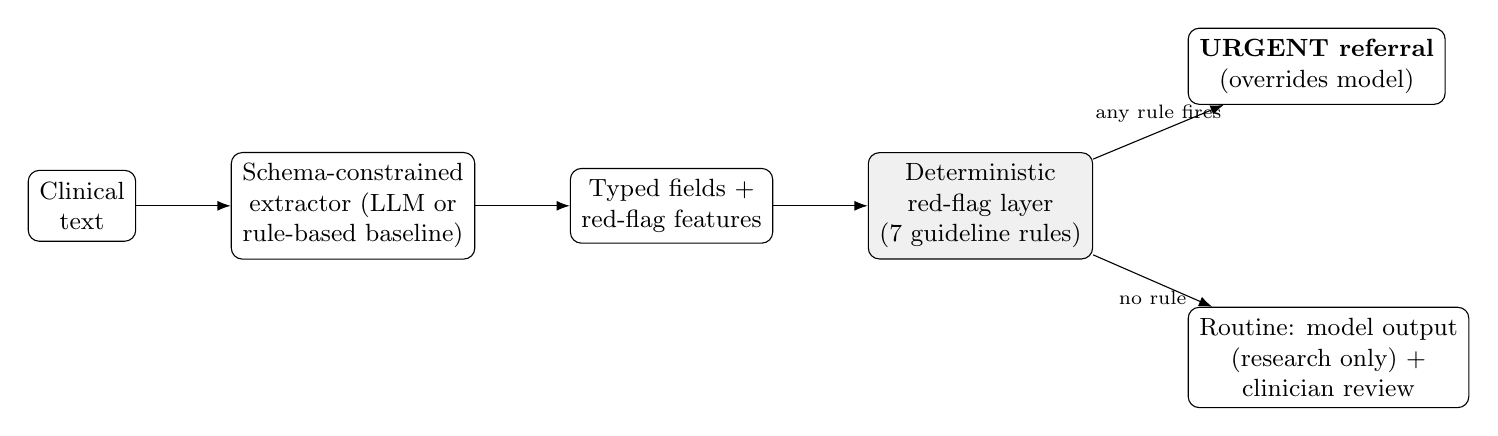
\begin{tikzpicture}[
  node distance=8mm and 12mm, >=Latex,
  box/.style={draw, rounded corners, align=center, inner sep=4pt, font=\small, minimum height=9mm},
  safe/.style={draw, rounded corners, align=center, inner sep=4pt, font=\small, minimum height=9mm, fill=black!6},
]
\node[box] (text) {Clinical\\text};
\node[box, right=of text] (extract) {Schema-constrained\\extractor (LLM or\\rule-based baseline)};
\node[box, right=of extract] (feat) {Typed fields +\\red-flag features};
\node[safe, right=of feat] (safety) {Deterministic\\red-flag layer\\(7 guideline rules)};
\node[box, above right=6mm and 12mm of safety] (urgent) {\textbf{URGENT referral}\\(overrides model)};
\node[box, below right=6mm and 12mm of safety] (routine) {Routine: model output\\(research only) +\\clinician review};
\draw[->] (text) -- (extract);
\draw[->] (extract) -- (feat);
\draw[->] (feat) -- (safety);
\draw[->] (safety) -- node[above,font=\scriptsize]{any rule fires} (urgent);
\draw[->] (safety) -- node[below,font=\scriptsize]{no rule} (routine);
\end{tikzpicture}%
}
\caption{The deterministic red-flag layer is the last, authoritative stage: any guideline red flag forces urgent referral and overrides probabilistic output. The extractor may be an open LLM (e.g., MedGemma) or the reproducible rule-based baseline evaluated here.}
\label{fig:arch}
\end{figure}

\subsection{Guideline-derived red-flag rules}
Seven rules encode time-critical presentations from the SSNHL and tinnitus guidelines \cite{chandrasekhar2019ssnhl,tunkel2014cpg}: (1) sudden hearing loss; (2) rapidly progressive loss; (3) unilateral sudden symptom; (4) acute aural fullness with a sudden drop; (5) single-sided tinnitus \emph{with} audiometric asymmetry (a combined rule); (6) vertigo; and (7) a focal neurologic sign. The decision is a logical OR across rules; combined rules require all their indicators. The rules are intentionally conservative---a missed red flag (a false negative) is the costly error---and deterministic, so their behavior is fully auditable and reproducible.

\subsection{Governance}
The extractor is constrained to a fixed schema with typed fields; free-text generation is disallowed for structured outputs, every field carries a rule-based reliability flag (source-span agreement, \emph{not} the model's token probability), and every field is clinician-verified before entering analysis. The safety layer supplements, never replaces, clinical assessment: a finite-set sensitivity of 1.00 is a target, not a guarantee of zero deployment misses.

\subsection{Open benchmark (no patient data)}
Because clinical text requires IRB approval and deidentification, the benchmark is entirely expert-authored or synthetic and can be released openly. It contains 71 cases: 34 \emph{structured} cases (19 guideline-urgent, 15 benign) whose gold urgency is assigned a priori from the guidelines \emph{independently} of the rule code, and 37 \emph{free-text} notes (18 urgent, 19 benign) spanning four categories---\emph{typical} (clean phrasing), \emph{negation} (explicit negatives), \emph{colloquial} (lay phrasing), and \emph{ambiguous} (vague onset/laterality)---including cases where an urgent presentation is described \emph{without} canonical keywords and resolved \emph{historical} events phrased with red-flag words. Each case carries laterality/onset/vertigo metadata for subgroup analysis.

\subsection{Two-level evaluation}
We evaluate at two levels. \textbf{Rule coverage} applies the deterministic layer to the correctly-extracted structured features, testing whether the rule set flags every guideline red flag and avoids over-flagging benign presentations. \textbf{End-to-end} runs each free-text note through the schema-constrained rule-based extractor and then the safety layer, so extraction error can propagate. Red-flag recall (sensitivity) is the safety-critical metric; we also report specificity and over-referral, with 95\% Wilson confidence intervals, and per-note-category performance.

\subsection{Three-system extractor comparison}
We compare three deliberately contrasting systems on the same 37 notes: (i) a naive keyword reference (v1), (ii) an improved deterministic reference (v2) adding historical/resolved-context suppression, colloquial and implicit-laterality cues, and keyword co-occurrence, and (iii) the independently developed medical LLM \texttt{google/medgemma-4b-it}. The first two bracket transparent under- and over-tuning behavior; the third tests whether the extraction bottleneck survives a change in model family and authorship. Neither rule system is presented as state of the art, and v2 is explicitly an \emph{in-sample, benchmark-tuned upper reference}, not an external-validation result.

The open-LLM path is implemented, not hypothetical: \texttt{llm\_medgemma.py} loads the 4-billion-parameter instruction-tuned checkpoint through \texttt{transformers}, uses a single zero-shot prompt, greedy decoding (temperature effectively zero), and at most 256 newly generated tokens, constrains output to the fixed extraction schema, and parses JSON robustly (code-fence/prose tolerant, brace-balanced, with a conservative all-\emph{unknown} fallback that can only \emph{under}-flag). No examples, benchmark cue lists, or gold labels are included in the prompt, and there is no model-specific post-processing. A schema-to-feature adapter maps all three systems to the same boolean red-flag features, after which \texttt{run\_llm\_eval.py} applies one identical metric implementation. We report per-feature precision/recall/F1, document-level exact feature match, urgency-changing error rate (an extraction error that flips the layer's decision), run-to-run consistency, and end-to-end sensitivity/specificity with Wilson intervals. Each run now emits a benchmark SHA-256 fingerprint and case-level gold and predicted features and urgency decisions. This audit artifact permits paired error analysis and detects benchmark drift; model text generations are not released and should be retained separately by future clinical-data custodians under their governance policy.

\section{Results}
\subsection{The deterministic layer: complete coverage, extraction-bounded end-to-end}
On correctly-extracted features the layer flagged every guideline red flag and over-referred none: sensitivity 100\% (19/19) and specificity 100\% (15/15) (Table~\ref{tab:redflag_results}). This confirms \emph{rule coverage}---the seven rules span the guideline red-flag taxonomy, and the combined single-sided-tinnitus-with-asymmetry rule correctly leaves benign single-sided tinnitus unflagged.

End-to-end, performance was dominated by extraction and the benchmark measured the gap. The \emph{naive} extractor achieved only 56\% recall (10/18) at 89\% specificity, missing eight urgent presentations phrased without canonical cues (e.g., ``\emph{my right ear stopped working after the flight}''; ``\emph{felt dizzy and my hearing cut out on one side}'') and false-alarming on resolved historical events. The \emph{improved} extractor reached 100\% recall and 100\% specificity \emph{on this benchmark} (Table~\ref{tab:redflag_results}), recovering the colloquial and ambiguous cases and suppressing historical false alarms (recall by category rose from 43\% to 100\% for colloquial and 33\% to 100\% for ambiguous notes; Table~\ref{tab:redflag_bycat}). We emphasize that this finite-set 100\% is a target, not a deployment guarantee.

\begin{table}[htbp]
\centering
\caption{\textbf{Deterministic referral-safety layer on the open benchmark} (34 structured + 37 text cases; author-curated/synthetic, no patient data). Sensitivity is red-flag recall (the safety-critical metric); 95\% Wilson CIs. \emph{Structured} evaluates rule coverage on correctly-extracted features; \emph{end-to-end} runs free text through a rule-based extractor first, so the benchmark discriminates extractor quality (v1 vs.\ the improved v2). Generated by \texttt{code/src/run\_redflag\_eval.py}.}
\label{tab:redflag_results}
\small
\resizebox{\textwidth}{!}{%
\begin{tabular}{lccccc}
\toprule
Evaluation & Pos. & Neg. & Sensitivity (95\% CI) & Specificity (95\% CI) & Over-referral \\
\midrule
Structured (rule coverage) & 19 & 15 & 100\% (83--100) & 100\% (80--100) & 0\% \\
End-to-end, rule-based v1 & 18 & 19 & 56\% (34--75) & 89\% (69--97) & 11\% \\
End-to-end, rule-based v2 (improved) & 18 & 19 & 100\% (82--100) & 100\% (83--100) & 0\% \\
\bottomrule
\end{tabular}}
\end{table}

\input{tables/table_redflag_bycat}

\subsection{Extraction baseline}
Field-level metrics track the end-to-end gap (Table~\ref{tab:llm_compare}): the naive extractor reached macro-F1 0.72 with a 27\% urgency-changing error rate, while the improved extractor reached macro-F1 0.94 with a 0\% urgency-changing error rate on this benchmark; both were perfectly reproducible (run-to-run consistency 1.00). Per feature (improved extractor; Table~\ref{tab:extraction}), detection was strong across the safety-relevant fields. Two structural gaps we previously flagged---the extraction \emph{schema} not encoding audiometric \emph{asymmetry} or a \emph{rapidly-progressive} course---have since been closed: the schema now carries an \texttt{audiometric\_asymmetry} field and a \texttt{rapidly\_progressive} course value, and the adapter maps both to their red-flag features (verified by unit tests), so an LLM mapped through the adapter no longer inherits those blind spots. The rule-based baseline numbers are unaffected (the adapter feeds only the LLM path).

\begin{table}[htbp]
\centering
\caption{\textbf{Per-feature detection by the improved rule-based extractor (v2)} on the 37-note benchmark (positive class = feature present). The improved extractor is an in-sample, benchmark-tuned reference rather than an external comparator. Generated by \texttt{code/src/run\_extraction\_eval.py}.}
\label{tab:extraction}
\small
\begin{tabular}{lcccc}
\toprule
Feature & Prec. & Rec. & F1 & Support \\
\midrule
Sudden hearing loss & 0.82 & 1.00 & 0.90 & 9 \\
Rapidly progressive loss & 0.80 & 1.00 & 0.89 & 4 \\
Unilateral acute symptom & 1.00 & 0.93 & 0.97 & 15 \\
Acute aural fullness & 1.00 & 1.00 & 1.00 & 4 \\
Single-sided tinnitus & 1.00 & 0.60 & 0.75 & 5 \\
Asymmetric hearing & 1.00 & 1.00 & 1.00 & 2 \\
Vertigo & 1.00 & 1.00 & 1.00 & 4 \\
Focal neurologic sign & 1.00 & 1.00 & 1.00 & 1 \\
\midrule
\textbf{Macro average} & 0.95 & 0.94 & 0.94 & \\
\bottomrule
\end{tabular}
\end{table}


\subsection{Open medical-LLM (MedGemma) evaluation}
The open-LLM comparison is not a promise but a measurement. A single command scores every extractor---the two rule-based references and an actual open medical LLM, \texttt{google/medgemma-4b-it}---through the identical benchmark, adapter, and metrics (we ran MedGemma on a free-tier GPU with greedy, deterministic decoding):
\begin{quote}\footnotesize\ttfamily
python src/run\_llm\_eval.py --extractor medgemma \textbackslash\\
\phantom{xx}--model google/medgemma-4b-it \textbackslash\\
\phantom{xx}--out ../paper02/outputs/llm\_extractor\_eval.json
\end{quote}
\begin{table}[htbp]
\centering
\caption{\textbf{Extractor comparison through the identical safety harness.} MedGemma used the same author-curated benchmark and schema adapter as the rule references but did not receive their cue lists. The tuned rule extractor is an in-sample reference, and this descriptive comparison is not an external validation or powered model ranking. Generated by \texttt{code/src/run\_llm\_eval.py}.}
\label{tab:llm_compare}
\small
\resizebox{\textwidth}{!}{%
\begin{tabular}{lcccccc}
\toprule
Extractor & Macro F1 & Doc.\ exact & Urg.-chg.\ err. & E2E recall & E2E spec. & Run consist. \\
\midrule
Rule-based v1 & 0.72 & 0.59 & 0.27 & 56\% & 89\% & 1.00 \\
Rule-based v2 (improved) & 0.94 & 0.84 & 0.00 & 100\% & 100\% & 1.00 \\
MedGemma (open LLM) & 0.75 & 0.57 & 0.11 & 78\% & 100\% & 1.00 \\
\bottomrule
\end{tabular}}
\end{table}

Through this harness, MedGemma reached \textbf{78\% end-to-end red-flag recall} (14/18; 95\% Wilson CI 55--91\%) at \textbf{100\% specificity} (19/19; over-referral 0\%), with field-level macro-F1 0.75 and a 10.8\% urgency-changing error rate; greedy decoding made it perfectly reproducible (run-to-run consistency 1.00). It therefore sits \emph{between} the two rule-based references---naive 56\%, MedGemma 78\%, tuned 100\%---on identical cases (Table~\ref{tab:llm_compare}). Its four missed urgent notes were the implicitly-phrased ones: recall was 88\% on typical phrasing but fell to 71\% (colloquial) and 67\% (ambiguous), the same categories where the naive rule extractor failed. Notably, although MedGemma \emph{over}-asserted audiometric asymmetry at the field level (precision 0.13, liberally reading ``asymmetry'' from narrative text), this did not produce a single over-referral: the conservative combined rule---single-sided tinnitus \emph{with} asymmetry---absorbed the over-call, a direct validation of the combined-rule design. The plumbing itself is separately checked by eight unit tests that exercise the full path (prompt construction, generation, code-fence/prose-tolerant JSON parsing, schema-to-feature mapping, safety layer, metrics) with a deterministic no-model stand-in.

This is a descriptive small-sample comparison, not a model-ranking exercise. The sensitivity point estimates differ by 22 percentage points between each adjacent system, but the corresponding Wilson intervals are wide and paired significance testing would be underpowered with only 18 urgent notes. We therefore report numerators, denominators, and intervals rather than claiming superiority. The clinically relevant finding is qualitative and consistent across field- and decision-level metrics: changing the extractor changes whether urgent cases reach the non-overridable layer.

MedGemma adds a useful change of extractor family and authorship: it neither authored the benchmark nor received its cue lists in the prompt. This reduces, but does not eliminate, circularity because the cases and gold annotations remain author-curated and public. Its intermediate result shows that the benchmark is not trivially saturated by this model under this prompt. It cannot establish that 78\% is the expected deployment performance, nor can one model constitute external validation. Independent annotation, additional frozen models, and real clinical notes are required for those claims.

\section{Discussion}
The central result is a clean separation of concerns. On this finite challenge set, the deterministic layer matched every gold decision when supplied gold features and exposed every fired rule for audit. Architecturally, once an affirmative feature reaches this last stage, a lower probabilistic score cannot cancel its referral message. This is the property a safety-critical otology pipeline needs, and it is achieved without a model. But end-to-end safety is governed by the extraction step, and the benchmark \emph{measures} how much: red-flag recall was 56\% (naive extractor), 78\% for an independently developed medical LLM (MedGemma-4b-it), and 100\% (tuned extractor) on identical cases. A red flag the extractor never surfaces cannot be rescued by a downstream rule, and a resolved historical event can trigger a false alarm; the improvements that closed the rule-extractor gap were precisely historical-context suppression and better handling of colloquial and implicit phrasing---and MedGemma's own misses fell in exactly those colloquial/ambiguous categories, so the bottleneck is intrinsic to extraction, not an artifact of one hand-written extractor.

The practical implications are specific. First, \textbf{extraction quality---not the rule layer---is the safety bottleneck}, and an open benchmark that quantifies it (as this one does, spanning 56\%, 78\%, and 100\% recall across three extractor configurations) is a prerequisite for trustworthy deployment. Second, \textbf{a finite-set recall of 100\% is a target, not a guarantee}: the tuned extractor is perfect \emph{on these 71 curated cases}, but an off-the-shelf open medical LLM reaches only 78\% on the same cases, and real notes are messier still. \textbf{Mandatory clinician verification of the extracted red-flag features is therefore load-bearing, not a formality}---the layer plus human-in-the-loop review, not the layer alone, is the safe configuration; a model at 78\% recall would, unverified, let roughly one urgent case in five reach the ``routine'' path. The measured MedGemma result also makes the bar concrete: an off-the-shelf open LLM, plugged into the same harness, does not yet match the tuned extractor and must improve on colloquial/ambiguous phrasing---the axes on which both it and the naive extractor failed---before it could be trusted without human review.

\subsection{Limitations}
This is a curated benchmark (71 cases), so confidence intervals are wide---MedGemma's 78\% recall carries a 55--91\% Wilson interval---and subgroup counts are modest; the benchmark is designed to be extended, and the harness supports arbitrarily many cases. The MedGemma evaluation, though real, uses the 4B instruction-tuned checkpoint under zero-shot schema prompting on the \emph{open} benchmark; larger MedGemma variants, few-shot prompting, and---above all---\emph{real} clinical notes (which need IRB-approved, deidentified text) remain to be tested, and performance on messy real-world text may differ from these curated cases. The benchmark, metrics, and adapter were fixed before the model was run, reducing model-specific tuning; nevertheless, benchmark authorship, gold annotation, and analysis were not independently replicated. The tuned extractor's perfect recall is in-sample, and neither it nor MedGemma's 78\% estimates deployment performance. Cases are English-language; multilingual and real-note robustness (including real negation and temporal complexity) remain to be tested. Finally, a finite-set recall of 1.00 at the rule-coverage level is a target, not a guarantee of zero deployment misses; the layer supplements, never replaces, clinical judgment.

\section{Conclusion}
A deterministic, guideline-derived safety layer can make an affirmative extracted red flag non-overridable and auditable; on this finite benchmark, it matched every gold decision when supplied gold features. But end-to-end safety is only as good as the extraction that feeds it: on free text, red-flag recall was 56\%, 78\%, and 100\% across a naive extractor, a real open medical LLM (MedGemma-4b-it), and a tuned extractor on identical cases, so extraction quality is the safety bottleneck and clinician verification is essential. By releasing the rules, challenge set, reproducible extractors, schema-to-feature adapter, metrics, benchmark fingerprint, and case-level audit trail, we turn a safety claim into an inspectable evaluation. The MedGemma result partially probes, but does not resolve, the circularity of a self-authored benchmark; independent annotation and clinical-note validation remain necessary.

\section*{Declarations}
\textbf{Corresponding Author:} Geunsik Lim, Sungkyunkwan University, Republic of Korea; \texttt{leemgs@g.skku.edu}; ORCID \href{https://orcid.org/0000-0003-1845-7132}{0000-0003-1845-7132}. \textbf{Author Contributions (CRediT):} \emph{Geunsik Lim}---Conceptualization, Methodology, Software, Formal analysis, Writing (original draft \& editing), Visualization. The author read and approved the manuscript. \textbf{Data and Code Availability:} The benchmark, deterministic rules, rule-based extractors, the open medical-LLM (MedGemma) extractor path, the unified evaluation harness, benchmark fingerprinting, case-level decision audit output, its end-to-end tests, and the generated result tables are openly available in the STARS repository (\texttt{code/src/redflag\_benchmark.py}, \texttt{safety.py}, \texttt{llm\_extract.py}, \texttt{llm\_medgemma.py}, \texttt{run\_redflag\_eval.py}, \texttt{run\_extraction\_eval.py}, \texttt{run\_llm\_eval.py}, \texttt{test\_llm\_medgemma.py}), together with a ready-to-run free-GPU notebook (\texttt{code/notebooks/medgemma\_eval\_colab.ipynb}) that reproduces the MedGemma row on a free Colab/Kaggle T4. No patient data are used or redistributed. \textbf{Ethics:} No human-subjects data; all cases are expert-authored or synthetic. A prospective clinical evaluation will proceed only under IRB approval. \textbf{AI-Use Disclosure:} Generative AI tools assisted in drafting and code scaffolding; the author reviewed and is responsible for all content. In any clinical use, open medical LLMs are confined to clinician-verified extraction and never make autonomous decisions. \textbf{Conflicts of Interest:} None declared. \textbf{Funding:} None.

% References follow the ICMJE/Vancouver style required by JAMIA: numbered in the
% order of first citation in the text.
\begin{thebibliography}{9}
\bibitem{chandrasekhar2019ssnhl} Chandrasekhar SS, Tsai Do BS, Schwartz SR, et al. Clinical practice guideline: sudden hearing loss (update). \textit{Otolaryngol Head Neck Surg}. 2019;161(1\_suppl):S1--S45. \url{https://doi.org/10.1177/0194599819859885}
\bibitem{tunkel2014cpg} Tunkel DE, Bauer CA, Sun GH, et al. Clinical practice guideline: tinnitus. \textit{Otolaryngol Head Neck Surg}. 2014;151(2\_suppl):S1--S40. \url{https://doi.org/10.1177/0194599814545325}
\bibitem{agrawal2022llmextract} Agrawal M, Hegselmann S, Lang H, Kim Y, Sontag D. Large language models are few-shot clinical information extractors. In: \textit{Proceedings of the 2022 Conference on Empirical Methods in Natural Language Processing (EMNLP)}. Association for Computational Linguistics; 2022:1998--2022. \url{https://doi.org/10.18653/v1/2022.emnlp-main.130}
\bibitem{uzuner2010i2b2} Uzuner \"{O}, South BR, Shen S, DuVall SL. 2010 i2b2/VA challenge on concepts, assertions, and relations in clinical text. \textit{J Am Med Inform Assoc}. 2011;18(5):552--556. \url{https://doi.org/10.1136/amiajnl-2011-000203}
\bibitem{singhal2023llmclinical} Singhal K, Azizi S, Tu T, et al. Large language models encode clinical knowledge. \textit{Nature}. 2023;620(7972):172--180. \url{https://doi.org/10.1038/s41586-023-06291-2}
\bibitem{medgemma2025blog} Google Research. MedGemma: open models for health AI development. 2025. Accessed August 8, 2026. \url{https://research.google/blog/medgemma-our-most-capable-open-models-for-health-ai-development/}
\bibitem{medgemma2026docs} Google Health AI Developer Foundations. MedGemma. 2026. Accessed August 8, 2026. \url{https://developers.google.com/health-ai-developer-foundations/medgemma}
\bibitem{wong2021sepsis} Wong A, Otles E, Donnelly JP, et al. External validation of a widely implemented proprietary sepsis prediction model in hospitalized patients. \textit{JAMA Intern Med}. 2021;181(8):1065--1070. \url{https://doi.org/10.1001/jamainternmed.2021.2626}
\bibitem{finlayson2021datashift} Finlayson SG, Subbaswamy A, Singh K, et al. The clinician and dataset shift in artificial intelligence. \textit{N Engl J Med}. 2021;385(3):283--286. \url{https://doi.org/10.1056/NEJMc2104626}
\bibitem{collins2024tripodai} Collins GS, Moons KGM, Dhiman P, et al. TRIPOD+AI statement: updated guidance for reporting clinical prediction models that use regression or machine learning methods. \textit{BMJ}. 2024;385:e078378. \url{https://doi.org/10.1136/bmj-2023-078378}
\end{thebibliography}

\end{document}
